
During the design phase of a program test oracles are usually available.
However, this is not the case during the operational stage of a program.
We do need some form of error detection for the SFL technique to work.
To facilitate debugging of a program in this stage we would like to have
a test oracle as in the design state, however this would require automatic
generation of invariants based on the program specifications, which is 
hard and currently not done in practice.
Also, the detailed program specifications needed to achieve this are usually
unavailable.

Secondly, some program faults cause a crash of the program,
or cause the program to hang at a certain point.
Next to that, determining correct execution is often more difficult than simply comparing outputs.
Examples of these programs are programs with buggy user interfaces,
continuous programs with sparse buffer overflow events, etcetera.
Implementing application-specific invariants to detect these bugs is an expensive task 
and very error-prone and often incomplete, as it is done manually.
Rather, we would like simple, generic program invariants,
which can be automatically trained to become application specific.
In combination with the fault localization techniques, 
this automatic error detection could ultimately evolve into
a fully automated fault localization,
given that a program is trained for normal behavior using the test oracle
during the design phase.


In the \verb|textVal| example (Section \ref{s:exampleProgram}), 
the first five test inputs result in an output which can easily be verified.
However, the sixth test input causes the program to hang.
No output is returned, so it can not be verified, 
although the behavior is such that we know that this run fails expected execution.
In normal cases, a \verb|^C| command will stop execution of the program,
but will update the spectrum data before shutting down to keep the important data of this failing run.
Because of the threaded nature of this program the program keeps blocking
and termination of the program is only possible with a kill signal.

To monitor programs for errors, the tool set is able to instrument programs to
automatically detect errors and stop the running program, while recording a failed run.
This is done by training certain program invariants and enabling screeners to trigger the fault.
Program invariants and fault screeners are discussed in the next sections.
Finally, the \verb|textVal| program is instrumented with an invariant type 
to demonstrate automatic error detection and to help find the second bug.


\section{Program Invariants}

	Program invariants are predicates that should hold throughout the execution of the program.
	For example, each loop in the program can hold an invariant which expresses the maximum number of iterations.
	During the training phase with expected behavior of the program, this maximum number is updated.
	During the testing phase, if the number of iterations exceeds the recorded value, 
	the program invariant is violated and an error is generated.

	The \verb|instrument| tool is able to instrument different types of invariants.
	A summary of these invariant types is given in Table \ref{t:programInvariants}.
	Each of these invariant types will be discussed in the next sections.

	\begin{table}
		\begin{center}
		\begin{tabular}{l|l}
			name & description \\
			\hline
			-invstore         & instrument store invariants \\
			-invload          & instrument load invariants \\
			-invlooploop      & instrument loop counter invariants \\
			-invfunctiontimer & instrument function timing invariants \\
		\end{tabular}
		\caption{instrumentation passes for program invariants}
		\label{t:programInvariants}
		\end{center}
	\end{table}


\subsection{Stores}

		Every time a value is written to memory this is monitored when the program is instrumented
		with the \verb|store| invariant type.
		If an unexpected value is stored (e.g., a value outside an array bound) according to the training phase,
		an error is generated.
	
		Performing instrumentation for the \verb|store| invariant type is done using the 
		\verb|-invstore| option of the \verb|instrument| tool.
		For example,\\
		\verb|  # instrument -invstore -bypassmain textVal.bc -o textVal.ibc|\\
		will instrument stores and will perform the necessary bypass of the main function.

\subsection{Loads}

		Every time a value is loaded from memory this is monitored when the program is instrumented
		with the \verb|load| invariant type.
		If an unexpected value is loaded (e.g., a NULL pointer), according to the training phase,
		an error is generated.	

		Performing instrumentation for the \verb|load| invariant type is done using the 
		\verb|-invload| option of the \verb|instrument| tool.
		For example,\\
		\verb|  # instrument -invload -bypassmain textVal.bc -o textVal.ibc|\\
		will instrument loads and will perform the necessary bypass of the main function.


\subsection{Loop Counters}

		The \verb|instrument| tool is able to get information of execution loops
		existing in the program
		and instrument it to count the number of consecutive iterations of each loop.
		Most of the time, these loops will have a limited number of iterations during execution.
		The \emph{normal} number of iterations can be trained when the program is run on input
		resulting in expected behavior.
		This invariant type is very useful for situations where unexpected endless loops occur
		causing the program to stop functioning.

		Performing instrumentation for the \verb|loop counter| invariant type is done using the 
		\verb|-invloopcount| option of the \verb|instrument| tool.
		For example,\\
		\verb|  # instrument -invloopcount -bypassmain textVal.bc -o textVal.ibc|\\
		will instrument the counting of loop iterations and will perform the necessary bypass of the main function.

	
\subsection{Function Timing}

		The instrumentation of the program supports timed invariants as well.
		The function timing invariant monitors the time that is spent within a function.
		A timer with a 1 ms interval signals an increment of every function which is \emph{active},
		i.e., which is still in the process of being executed.
		At the start of a function execution the counter is set to zero.
		During the training phase, every millisecond a program remains in a function this is recorded.
		If, during testing, the program remains in that function for longer than it should,
		an error is generated.

		Performing instrumentation for the \verb|function timing| invariant type is done using the 
		\verb|-invfunctiontimer| option of the \verb|instrument| tool.
		For example,\\
		\verb|  # instrument -invfunctiontimer -bypassmain \ | \\
		\verb|  > textVal.bc -o textVal.ibc|\\
		will instrument functions for timing and will perform the necessary bypass of the main function.


\subsection{Custom Invariant Instrumentation}

		As with the program spectra, 
		custom instrumentation passes can be created for instrumenting the program for other invariants.
		The technical information needed for implementing custom instrumentation passes 
		is discussed in detail in Appendix \ref{c:WritingInstrumentationPasses}.

		
	
\section{Fault Screeners}

	Fault screeners are used to train and monitor each variable that is instrumented as invariant.
	Different types of fault screeners exist, 
	determining the possible values an instrumented variable assumes.
	The invariant of the variable is that the variable remains within the trained set of values.
	The currently supported screeners are a range screener and a bit mask screener.
	These are discussed in the following sections.

\subsection{Range}

		When a range screener is enabled for an invariant, 
		the minimum and maximum values an instrumented variable obtains during training is recorded.
		If, during testing, the variable suddenly assumes a value outside of this range,
		an error is generated.

\subsection{Bit Mask}

		A bit mask screener monitors the actual bits of a variable.
		Bits that are changed during execution are marked in the training phase.
		If, in the testing phase, an unexpected bit is changed, an error is generated.

%\subsection{Bloom Filter}

%\section{Training and Testing}


\section{Automatic Error Detection in Practice}
	
	To demonstrate automatic error detection we will try to locate the second bug in the \verb|textVal|
	program.
	As mentioned previously, the sixth test input will cause the program to hang.
	This erratic behavior can be caught by instrumenting the program to generate an error if
	the program remains within a function for too long.
	The tool set offers the \verb|function timing| instrumentation for this purpose.
	The \verb|textVal| program will now be instrumented using the following commands.\\
	\verb|  # llvm-gcc -g -emit-llvm -c textVal.c -o textVal.bc| \\
	\verb|  # instrument -f -invfunctiontimer -spbasicblock \ | \\
	\verb|  > -bypassmain textVal.bc -o textVal.ibc| \\
	\verb|  # llc -f textVal.ibc -o textVal.s| \\
	\verb|  # gcc textVal.s -lpthread -linstrument -o textVal| \\

	The resulting executable must now be trained with normal behavior
	(i.e., input test data for which the program test is known to pass)
	to be able to detect abnormal behavior.
	To do this we simply execute the program with test inputs which not cause the program to hang.
	The instrumented program is in training mode by default.
	In other words we may use the same sequence of tests as before.
	But before that, the existing data file must be removed, 
	since it is not compatible with the newly instrumented version.
	The instrumented program will complain about this if it does find an existing incompatible data file.\\
	\verb|  # rm datafile.dat|\\
	\verb|  # ./textVal < test1.in|\\
	\verb|  # ./textVal < test2.in|\\
	\verb|  # ./textVal < test3.in|\\
	\verb|  # ./textVal < test4.in|\\
	\verb|  # ./textVal < test5.in|\\
	
	At this point the invariant is trained with expected values.
	This can be viewed and edited by the \verb|zoltar| tool.
	To do this, we start the \verb|zoltar| tool as discussed previously.
	In the main menu we select \verb|Invariants| to view all instrumented invariant types.
	We select the \verb|Function Timer| invariant and we will be presented with some options
	for modifying the invariant training values.
	We select \verb|Edit invariants| to view the trained values.
	
	With the \emph{left} and \emph{right} keys the trained values corresponding to the 
	\verb|range| screener and \emph|bit mask| screener can be viewed and edited.
	Also, the screeners can be enabled and disabled to the wishes of the user.
	This can be useful in cases in which you know that a value can assume any value,
	although this is not trained, e.g., random values or pointers.
	
	The trained values are very strict.
	In this case, the time spent in a function is related to the size of the input,
	which may vary.
	To be able to support a wider range of inputs, 
	we can stretch these values, introducing a safe margin.
	Only if an unexpected large amount of time is spent in a function we want an error to be generated.
	To return to the previous screen we press the \emph{backspace} key.
	We can now select the \verb|stretch 100% (MAX only)| option to double the range of the 
	valid number of milliseconds a function may be executed.
	After this is done, the new values are shown.
	To be sure, we will repeat this one more time, to get a very reasonable range of execution time.
	The resulting values are shown in the screenshot of the \verb|zoltar| program in 
	Figure \ref{fig:analyzeInv}.
	
	\begin{figure}[h!]
		\begin{center}
		\begin{tabular}{c}
			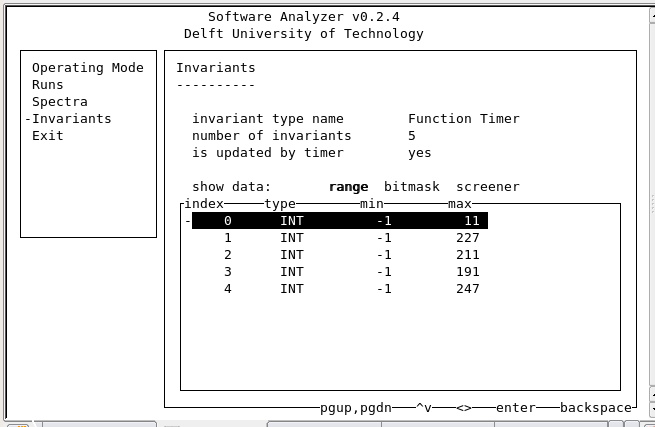
\includegraphics[scale=0.40]{sources/analyze_inv.png} \\
		\end{tabular}
		\end{center}
		\caption{Invariant training of the textVal program.}
		\label{fig:analyzeInv}
	\end{figure}

	Next, the program has to be set to testing mode in order to be able to detect and react upon an 
	error caused by an invariant violation.
	To do this, we press \emph{backspace} a number of times until the main menu is active.
	In the summary the operating mode is shown to be set to \verb|training|.
	We select \verb|Operating Mode| from the menu and select \verb|testing| to configure the program
	for automatic error detection.
	When this is done, we press the '\emph{q}' key or go to the main menu and select \emph{exit}.
	
	At this moment the instrumented program is trained and ready to handle invariant violations.
	Now we can test the sixth test input using the following command.\\
	\verb|  # ./textVal < test6.in|\\
	During the execution a range invariant has been violated and an error is generated accordingly.
	If the \verb|zoltar| tool is started again, the status of all runs can be examined.
	Select \verb|Runs| from the main menu and notice that the sixth run has automatically been 
	given the \emph{failed} status, because during that run an error occurred.
	Exit the \verb|zoltar| tool and start \verb|xzoltar| to perform SFL analysis
	and give visual feedback in the source code.
	
	\begin{figure}[h!]
		\begin{center}
		\begin{tabular}{c}
			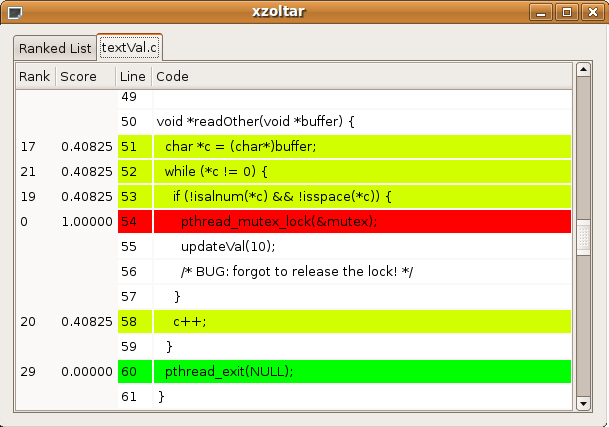
\includegraphics[scale=0.40]{sources/ganalyze_bug2.png} \\
		\end{tabular}
		\end{center}
		\caption{Visualization of the SFL result showing the location of the second bug.}
		\label{fig:ganalyzeBug2}
	\end{figure}

	The relevant piece of code according to the SFL results is given in Figure \ref{fig:ganalyzeBug2}.
	It shows that the basic block starting at line 54 in the code corresponds most with the run
	which resulted in an error.
	This is indeed within the function of the third thread scanning for non-alphanumeric characters.
	The actual block is the part which does lock the mutex, but does not unlock it.
	
	Using this tool set we are able to locate faults for various types of faults,
	including the rather difficult faults in which lines of code are missing, 
	as demonstrated in this tutorial.
	No knowledge about the software under test is required.
	The output of the tool can help software developers to investigate their code more efficiently,
	by being lead to the most probable locations at which the fault could be.
	
